%%%%%%%%%%%%%%%%%%%%%%%%%%%%%%%%%%%%%%%%%
% Academic Title Page
% LaTeX Template
% Version 2.0 (17/7/17)
%
% This template was downloaded from:
% http://www.LaTeXTemplates.com
%
% Original author:
% WikiBooks (LaTeX - Title Creation) with modifications by:
% Vel (vel@latextemplates.com)
%
% License:
% CC BY-NC-SA 3.0 (http://creativecommons.org/licenses/by-nc-sa/3.0/)
% 
% Instructions for using this template:
% This title page is capable of being compiled as is. This is not useful for 
% including it in another document. To do this, you have two options: 
%
% 1) Copy/paste everything between \begin{document} and \end{document} 
% starting at \begin{titlepage} and paste this into another LaTeX file where you 
% want your title page.
% OR
% 2) Remove everything outside the \begin{titlepage} and \end{titlepage}, rename
% this file and move it to the same directory as the LaTeX file you wish to add it to. 
% Then add \input{./<new filename>.tex} to your LaTeX file where you want your
% title page.
%
%%%%%%%%%%%%%%%%%%%%%%%%%%%%%%%%%%%%%%%%%

%----------------------------------------------------------------------------------------
%  PACKAGES AND OTHER DOCUMENT CONFIGURATIONS
%----------------------------------------------------------------------------------------

\documentclass[11pt]{article}

\usepackage[utf8]{inputenc} 
\usepackage[T1]{fontenc} 

\usepackage{mathpazo} % Palatino font

\usepackage{graphicx} 
\usepackage{hyperref}
\usepackage[spanish]{babel}
\usepackage{float}

\newcommand{\seclabel}[1]{\label{sec:#1}}
\newcommand{\figlabel}[1]{\label{fig:#1}}
\newcommand{\tablabel}[1]{\label{tab:#1}}
\newcommand{\chaplabel}[1]{\label{chap:#1}}
\newcommand{\figref}[1]{Figure~\ref{fig:#1}}
\newcommand{\secref}[1]{Section~\ref{sec:#1}}
\newcommand{\chapref}[1]{Chapter~\ref{chap:#1}}
\newcommand{\tabref}[1]{Table~\ref{fig:#1}}

\begin{document}

%----------------------------------------------------------------------------------------
%  TITLE PAGE
%----------------------------------------------------------------------------------------

\begin{titlepage} % Suppresses displaying the page number on the title page and the subsequent page counts as page 1
  \newcommand{\HRule}{\rule{\linewidth}{0.5mm}} % Defines a new command for horizontal lines, change thickness here
  
  \center % Centre everything on the page
  
  %------------------------------------------------
  %  Logo
  %------------------------------------------------

  \begin{figure}
    \centering
    
\includegraphics[width=0.5\linewidth]{./images/logos/BRC_SinFondo.png}
  \end{figure}

  %------------------------------------------------
  %  Title
  %------------------------------------------------
  
  \HRule\\[0.4cm]
  
  {\Huge\bfseries Beauchef Robotic Challenge}\\[0.4cm] % Title of your document
  {\LARGE\bfseries Reglas}
  \HRule\\[1.5cm]
  
  
  \vfill\vfill
  %------------------------------------------------
  %  Organization
  %------------------------------------------------

  {\Large\bfseries Organizan}

  \begin{figure}[h!]
    \centering
    \begin{minipage}{.24\textwidth}
      \centering
      
\includegraphics[width=\linewidth]{./images/logos/ieee.png}
    \end{minipage}%
    \begin{minipage}{.24\textwidth}
      \centering
      
\includegraphics[width=\linewidth]{./images/logos/comrob.png}
    \end{minipage}
    \begin{minipage}{.24\textwidth}
      \centering
      
\includegraphics[width=\linewidth]{./images/logos/fablab.jpg}
    \end{minipage}
    \begin{minipage}{.24\textwidth}
      \centering
      
\includegraphics[width=\linewidth]{./images/logos/ob.png}
    \end{minipage}
  \end{figure}

  
  \vfill\vfill\vfill % Position the date 3/4 down the remaining page
  %------------------------------------------------
  %  Date
  %------------------------------------------------
  
  
  {\large Version: \the\year} % Date, change the \today to a set date if you want to be precise
  
  %------------------------------------------------
  %  Logo
  %------------------------------------------------
  
  %\vfill\vfill
  %\includegraphics[width=0.2\textwidth]{placeholder.jpg}\\[1cm] % Include a department/university logo - this will require the graphicx package
   
  %----------------------------------------------------------------------------------------
  
  \vfill % Push the date up 1/4 of the remaining page
  
\end{titlepage}

%----------------------------------------------------------------------------------------

\section*{Acerca de}
Este es el libro oficial de reglas de la competencia de robótica Beauchef Robotic Challenge (BRC).

Basado en la categoría \emph{Robotrace} del torneo \emph{All Japan Micromouse Contest} y en la categoría \emph{Velocidad} de la \emph{Competencia Robótica UTFSM}.

Cualquier consulta, enviar un mail a: \href{mailto:beauchefrc@gmail.com}{beauchefrc@gmail.com}

\section*{Agradecimientos}

Queremos agradecer a los miembros de la Comunidad de Robótica, Fablab y IEEE UChile por adaptar las reglas y organizar la BRC.

También queremos agradecer a las siguientes instituciones por su colaboración en la realización de BRC:

\begin{itemize}
   \item \textbf{Facultad de Ingeniería y Ciencias (FCFM)} de la Universidad de Chile por el apoyo entregado para la realización de esta competencia. 
   \item  \textbf{Innovación y Robótica Estudiantil} de la Universidad Técnica Federico Santa María (UTFSM) por su invaluable apoyo en la creación de este libro y organización de BRC.
 \end{itemize} 


\section*{Changelog}

\begin{itemize}
  \item \textbf{Julio 2019}
  \begin{itemize}
    \item Cambiada forma de rondas para que quede igual a la versión de UTFSM: en lugar de realizar un intento y esperar a que todos los robots participantes terminen para completar el siguiente intento, ahora el robot debe realizar los 3 intentos de forma inmediata.
  \end{itemize}
  \item \textbf{Junio 2019}
  \begin{itemize}
    \item Cambio en el tamaño de robotracer: de alto tiene 20 [cm].
    \item Apertura de competencia otras universidades.
    \item Re-ordenamiento de secciones.
    \item Re-escritura de algunos puntos.
  \end{itemize}
  \item \textbf{Agosto 2018}
  \begin{itemize}
    \item Recopilación de las reglas de BRC'18 para la creación de este libro de reglas.
  \end{itemize}
\end{itemize}

\pagebreak

\section{Objetivo de la Competencia}

El objetivo de la competencia es recorrer un circuito en el menor tiempo posible utilizando un robot seguidor de líneas autónomo. Un robot que participa en esta competencia se denomina Robotracer \footnote{Un ejemplo del formato de la competencia se puede ver en el siguiente video: \href{https://www.youtube.com/watch?v=960e5Q_PhWg}{www.youtube.com/watch?v=960e5Q\_PhWg}}.

\section{Reglas de la Competencia}

\begin{enumerate}
  \item La proyección del Robotracer con respecto al escenario debe cubrir la línea del trayecto durante la carrera. Si el Robotracer se sale completamente se considerará como vuelta inválida.

  \item Cada competidor tiene 9 minutos para un máximo de 3 intentos, incluidos en este tiempo las reparaciones y vueltas completadas. Estos intentos son todos de forma continua (e.g, un equipo tiene 9 minutos para realizar 3 intentos, luego viene el siguiente equipo, luego el siguiente y así sucesivamente).

  \item Para cada intento, el Robotracer debe comenzar desde el área de Salida-Meta (ver \secref{course} para definición de área de Salida-Meta) en la dirección especificada.

  \item Al terminar el recorrido, el Robotracer debe detenerse automáticamente en el área de Salida-Meta por al menos 2 segundos, de lo contrario la vuelta será considerada como inválida.

  \item La vuelta más rápida será registrada como el tiempo oficial.

  \item El tiempo de vuelta se considera desde que el sensor de salida detecta el Robotracer y termina cuando el sensor de meta lo detecte. Además, el cuerpo entero del Robotracer debe estar dentro del área de Salida-Meta, en caso contrario el tiempo no será medido.

  \item Si el Robotracer se apaga o se queda detenido por más de 2 segundos mientras compite, se considerará como vuelta inválida.

  \item Si el Robotracer está en medio de un intento y se acaban los 9 minutos, se considerará como vuelta inválida.

  \item Las condiciones lumínicas, de temperatura y de humedad serán las dadas por el ambiente. Peticiones para ajustarlas no serán aceptadas.

  \item Después de dar como iniciada una vuelta, si el Robotracer no puede pasar de la línea de inicio, igualmente será considerada como una vuelta.

  \item Sólo dentro del tiempo reglamentario los competidores tienen permitido calibrar los sensores exclusivamente dentro del área de meta.

  \item Luego de que el recorrido sea revelado al público, el competidor tiene prohibido agregar información específica sobre éste al Robotracer.

  \item El competidor tiene prohibido tocar el Robotracer una vez iniciada la vuelta, a menos que sea solicitado o permitido por un juez de la competencia.

  \item El juez de la competencia tiene permiso para preguntar al competidor sobre su Robotracer si es necesario.

  \item El equipo que logre completar el circuito en el menor tiempo, será el ganador
\end{enumerate}


\section{Reglas del Robotracer}

\begin{enumerate}
  \item El Robotracer debe ser autónomo, exceptuando la zona de partida. Los competidores tiene prohibido controlar el robot de forma alámbrica o inalámbrica.

  \item Los competidores tienen prohibido añadir, remover, reemplazar o modificar el hardware o el software del Robotracer durante la ronda. Sin embargo, se permiten pequeñas reparaciones mecánicas como ajustar piezas que se suelten.

  \item El tamaño del Robotracer no puede exceder un largo de 25 [cm], ancho de 25 [cm] y alto de 20 [cm].

  \item El Robotracer no puede estar equipado con ningún mecanismo de sujeción que pudiera aumentar su agarre y/o dañar el escenario, tales como: químicos adherentes, púas en las ruedas, entre otros.
\end{enumerate}

\section{Reglas de los Competidores}

\begin{enumerate}
  \item Los competidores pueden participar en equipos de hasta 3 personas.

  \item El competidor tiene permitido limpiar el polvo y la suciedad de las ruedas del Robotracer usando cinta adhesiva o similar. Sin embargo no está permitido utilizar un disolvente o similar con el propósito de incrementar la fricción.

  \item Los competidores tienen prohibido cargar programas o reemplazar la memoria ROM durante la ronda. Tampoco está permitido enviar cualquier tipo de información al Robotracer desde una unidad de desarrollo o consola terminal que sea independiente de la unidad Robotracer.

  \item Los competidores tienen prohibido tocar el Robotracer durante la ronda a menos que tengan autorización de un juez.

  \item Se permiten competidores de cualquier universidad de Chile. Sin embargo, estos deben ser alumnos regulares de pregrado (los alumnos de postgrado no pueden participar). Sin embargo, se pueden hacer algunas excepciones, como por ejemplo: alumnos que realicen doble titulación con Magíster. Para ello, deben pedir autorización a nuestro correo: \href{mailto:beauchefrc@gmail.com}{beauchefrc@gmail.com}
\end{enumerate}

\section{Reglas del Escenario}
\seclabel{course}

\begin{enumerate}
  \item La superficie del escenario esta hecha de tableros de MDF negro (Ver \figref{course}). Las lineas del recorrido están hechas con cinta blanca de 19 [mm] de ancho. El largo máximo del recorrido es de 150 [m].

  \item El recorrido está compuesto de segmentos rectos y arcos y las líneas se pueden cruzar.

  \item El recorrido de la pista será secreto hasta iniciar la competencia. Los organizadores pueden cambiar la forma de la pista sin previo aviso. Todos los Robotracer competirán en la misma pista con la misma forma.

  \item El radio mínimo del arco de curvatura es de 10 [cm]. La distancia al punto de cambio de curvatura es sobre 10 [cm] (Ver \figref{curve}).

  \item Cuando las líneas se cruzan, el ángulo de la intersección es de $90^\circ \pm 5^\circ$ (Ver \figref{intersection}). Antes y después de la intersección hay 25 [cm] de línea recta.

  \item Se denominará área de Salida-Meta la zona comprendida a 20 [cm] a la derecha e izquierda entre la línea de salida y la de meta (Ver \figref{gate_area1}). En la línea de salida y de meta estarán situados el Portal de Salida y el Portal de Meta respectivamente. El ancho del portal es de 40 [cm] y su altura es de 25 [cm] (Ver \figref{gate}).

  \item La línea de salida y de meta estarán en una sección recta. La línea de meta estará dispuesta 1 [m] antes de la línea de salida. Los marcadores de salida y meta estarán situados al costado derecho de la línea del recorrido (Ver detalles en las \figref{gate_area1} y \figref{gate_area2}).

  \item Antes y después de las líneas de meta y salida hay al menos 25 [cm] de línea recta.

  \item Donde hay cambios de curvatura hay marcadores de esquina al costado izquierdo de la línea del recorrido (Ver \figref{curve}). 

  \item La superficie del escenario será plana. Pudiendo existir desniveles de 5 [mm] entre las planchas de madera.

  \item En algunos casos, los arcos de curvatura aparecen continuamente (Ver \figref{curve}).

  \item El escenario está construido con una precisión humana. Por lo tanto, pueden existir desniveles de 5 [mm] a los sumo. No se aceptarán reclamos sobre el agarre de la superficie.

  \item La posición del sensor de salida y de meta se muestran en la \figref{gate}. Estos son de tipo infrarrojo y se encuentran a 1 [cm] por sobre el suelo.
\end{enumerate}

\begin{figure}[H]
  \centering
  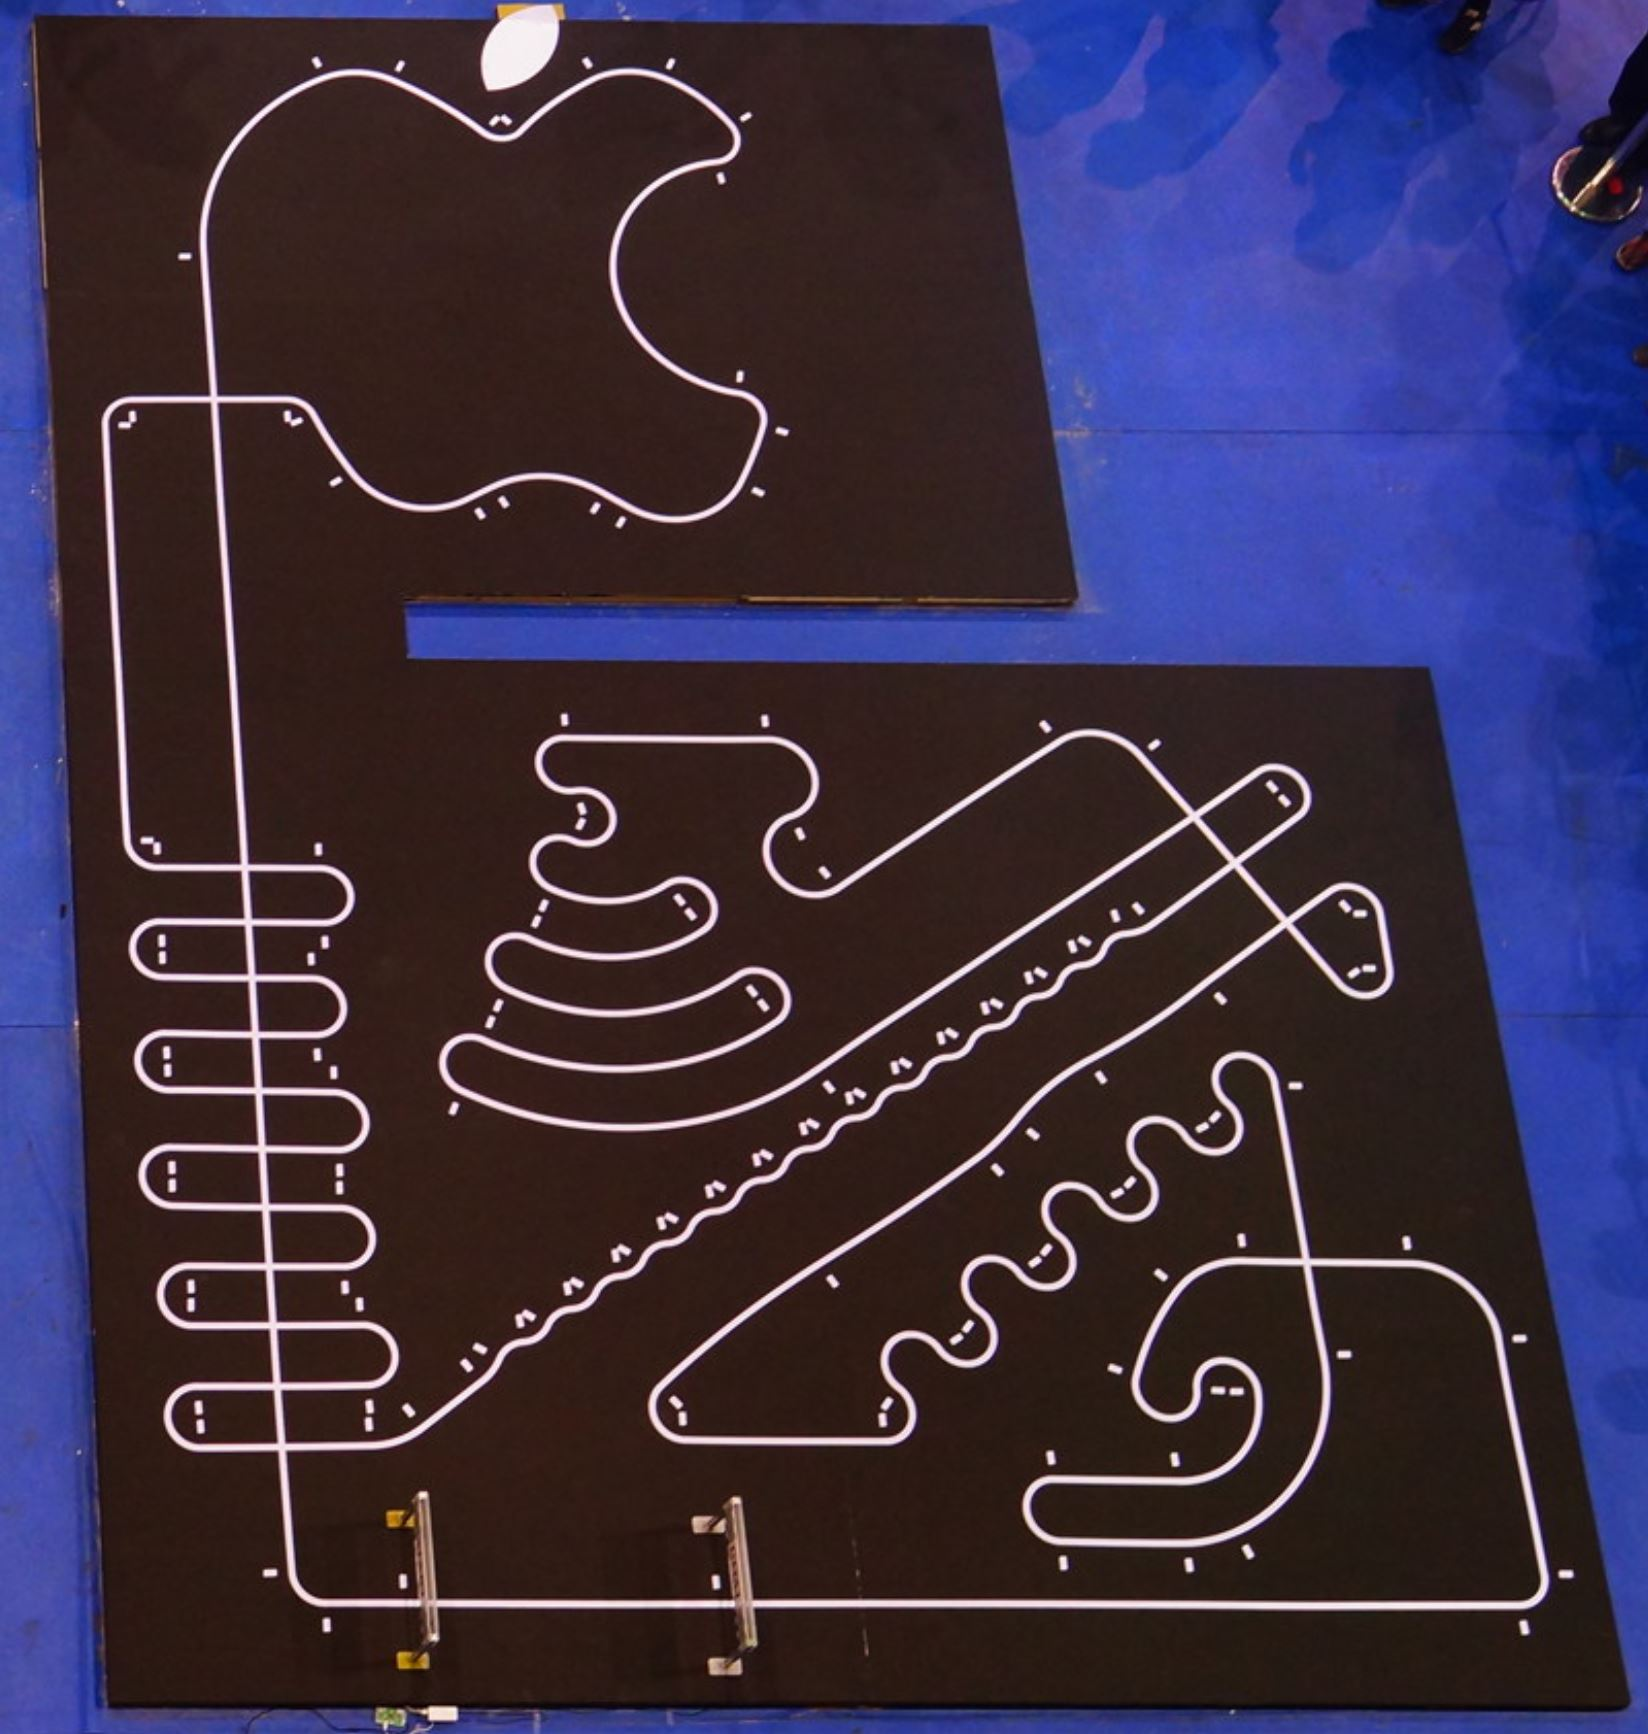
\includegraphics[width=\linewidth]{./images/rules/figure1.png}
  \caption{Pista Referencial}
  \figlabel{course}
\end{figure}

\begin{figure}[H]
  \centering
  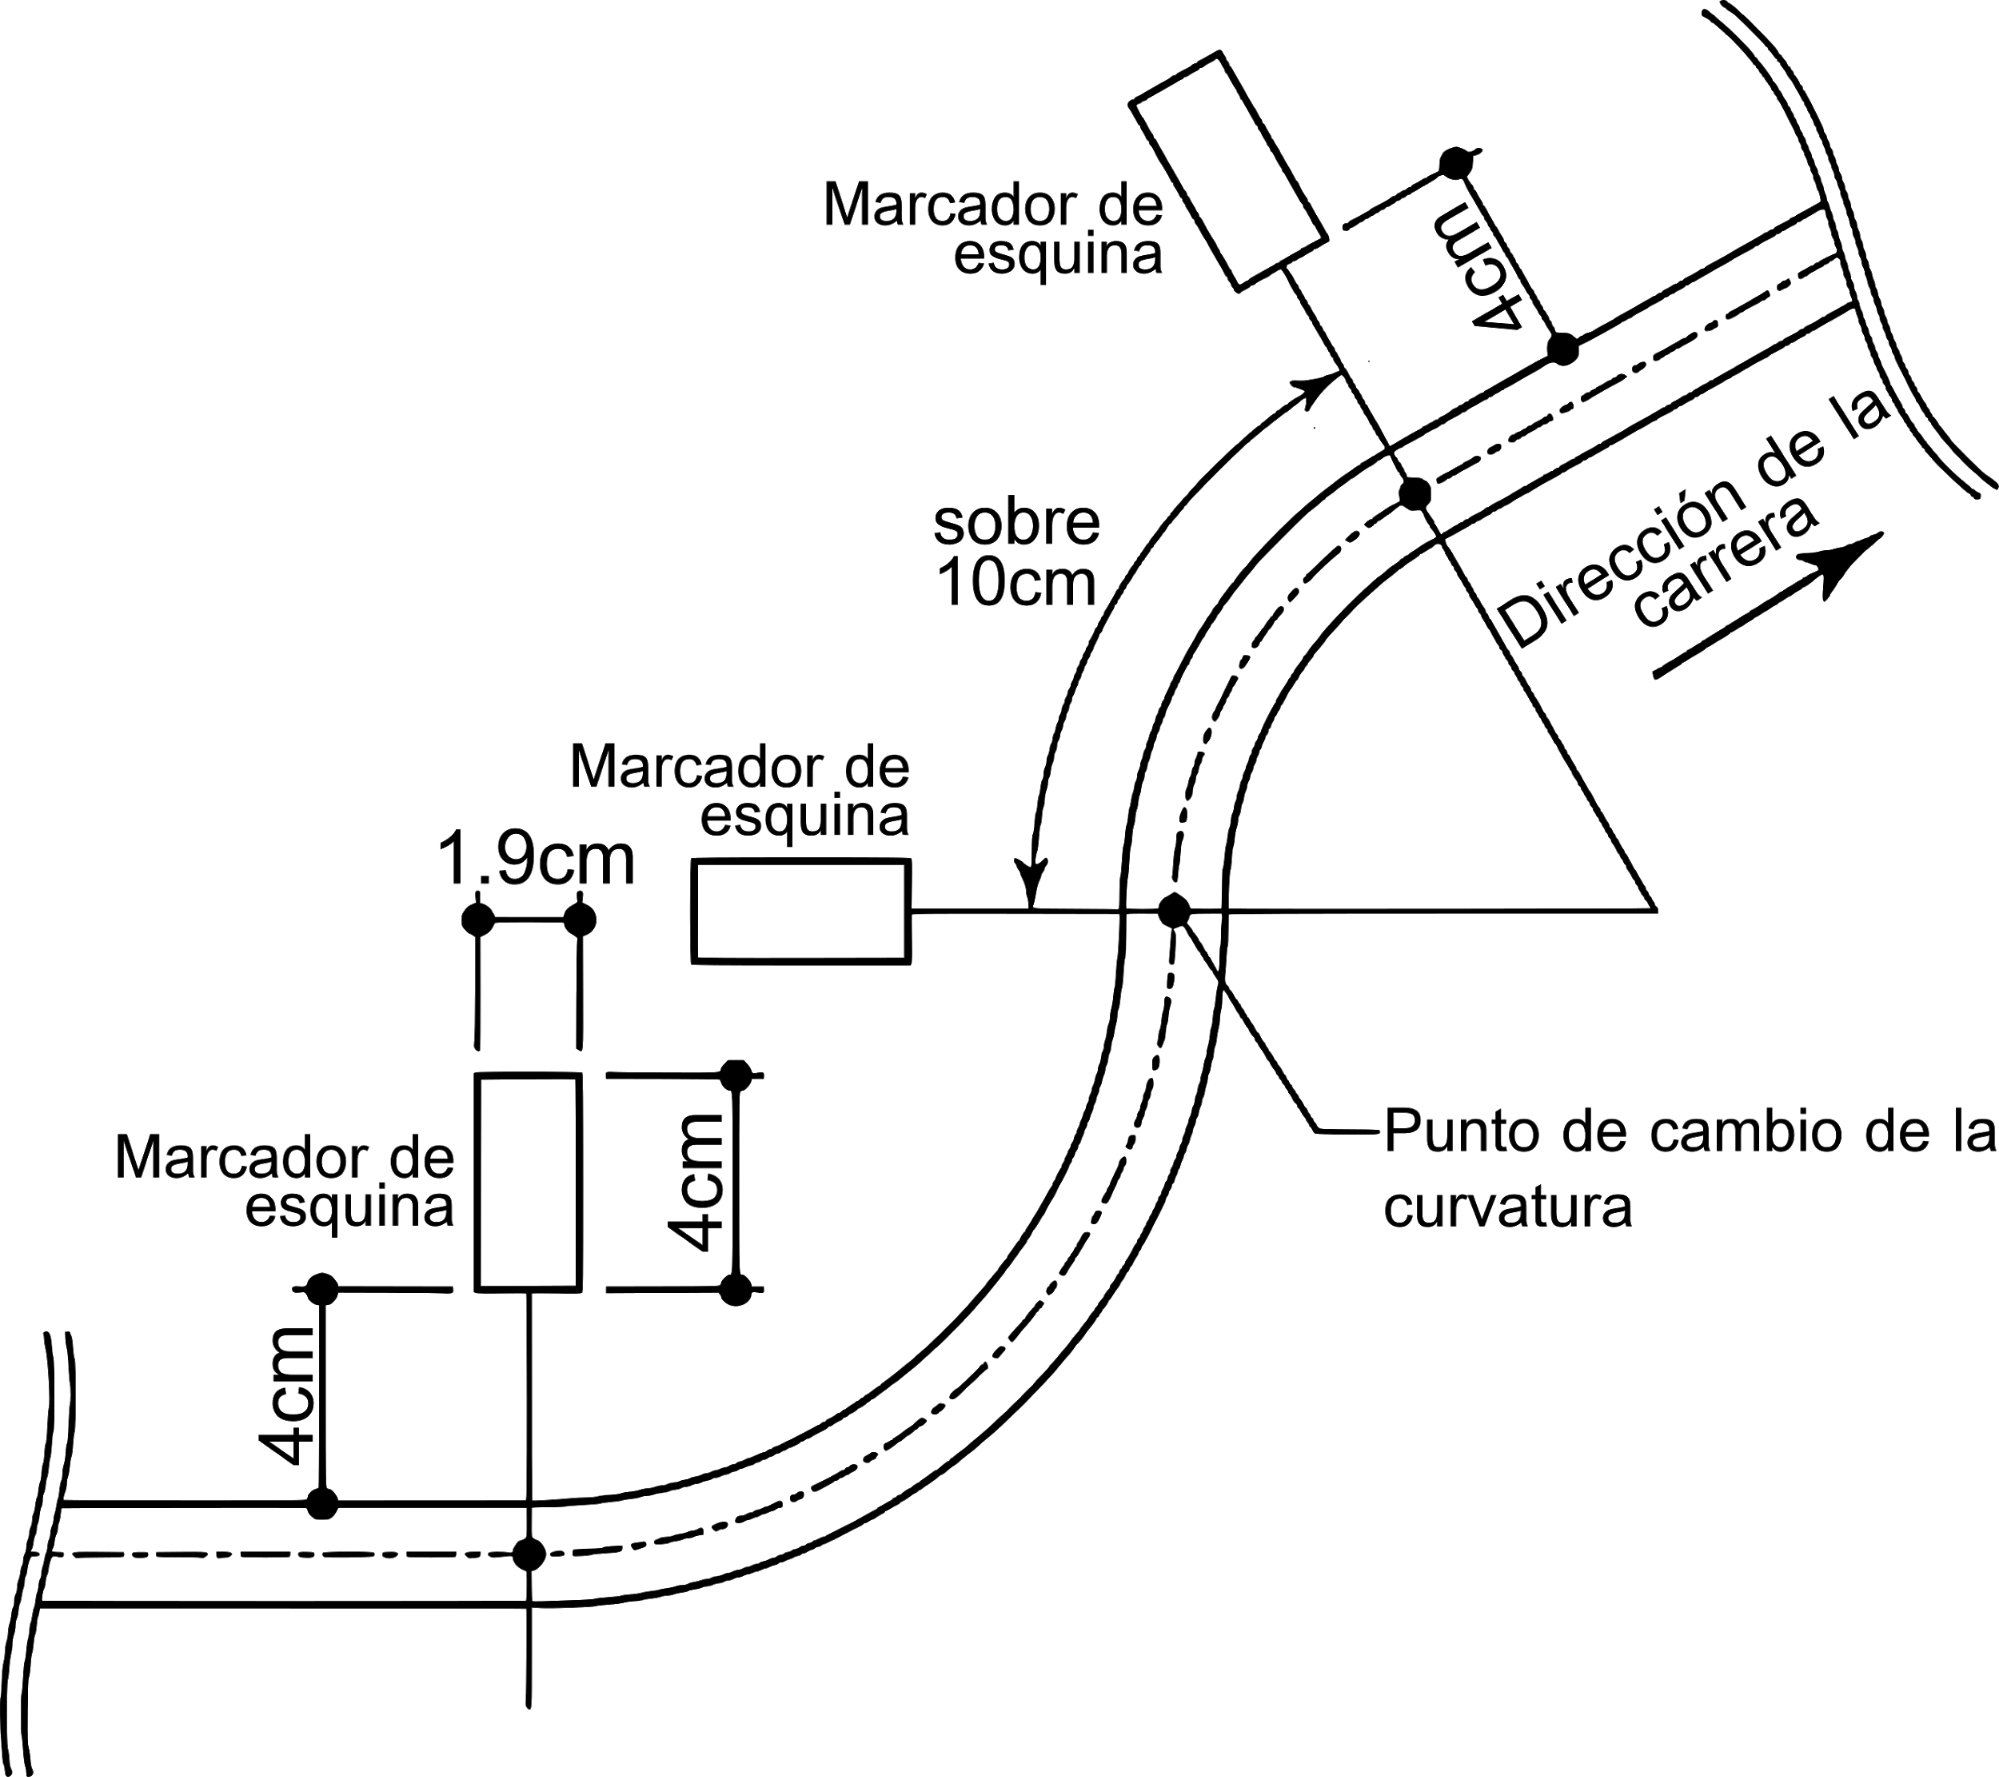
\includegraphics[width=0.6\linewidth]{./images/rules/figure2.png}
  \caption{Cambios de curvatura y marcadores de esquina}
  \figlabel{curve}
\end{figure}

\begin{figure}[H]
  \centering
  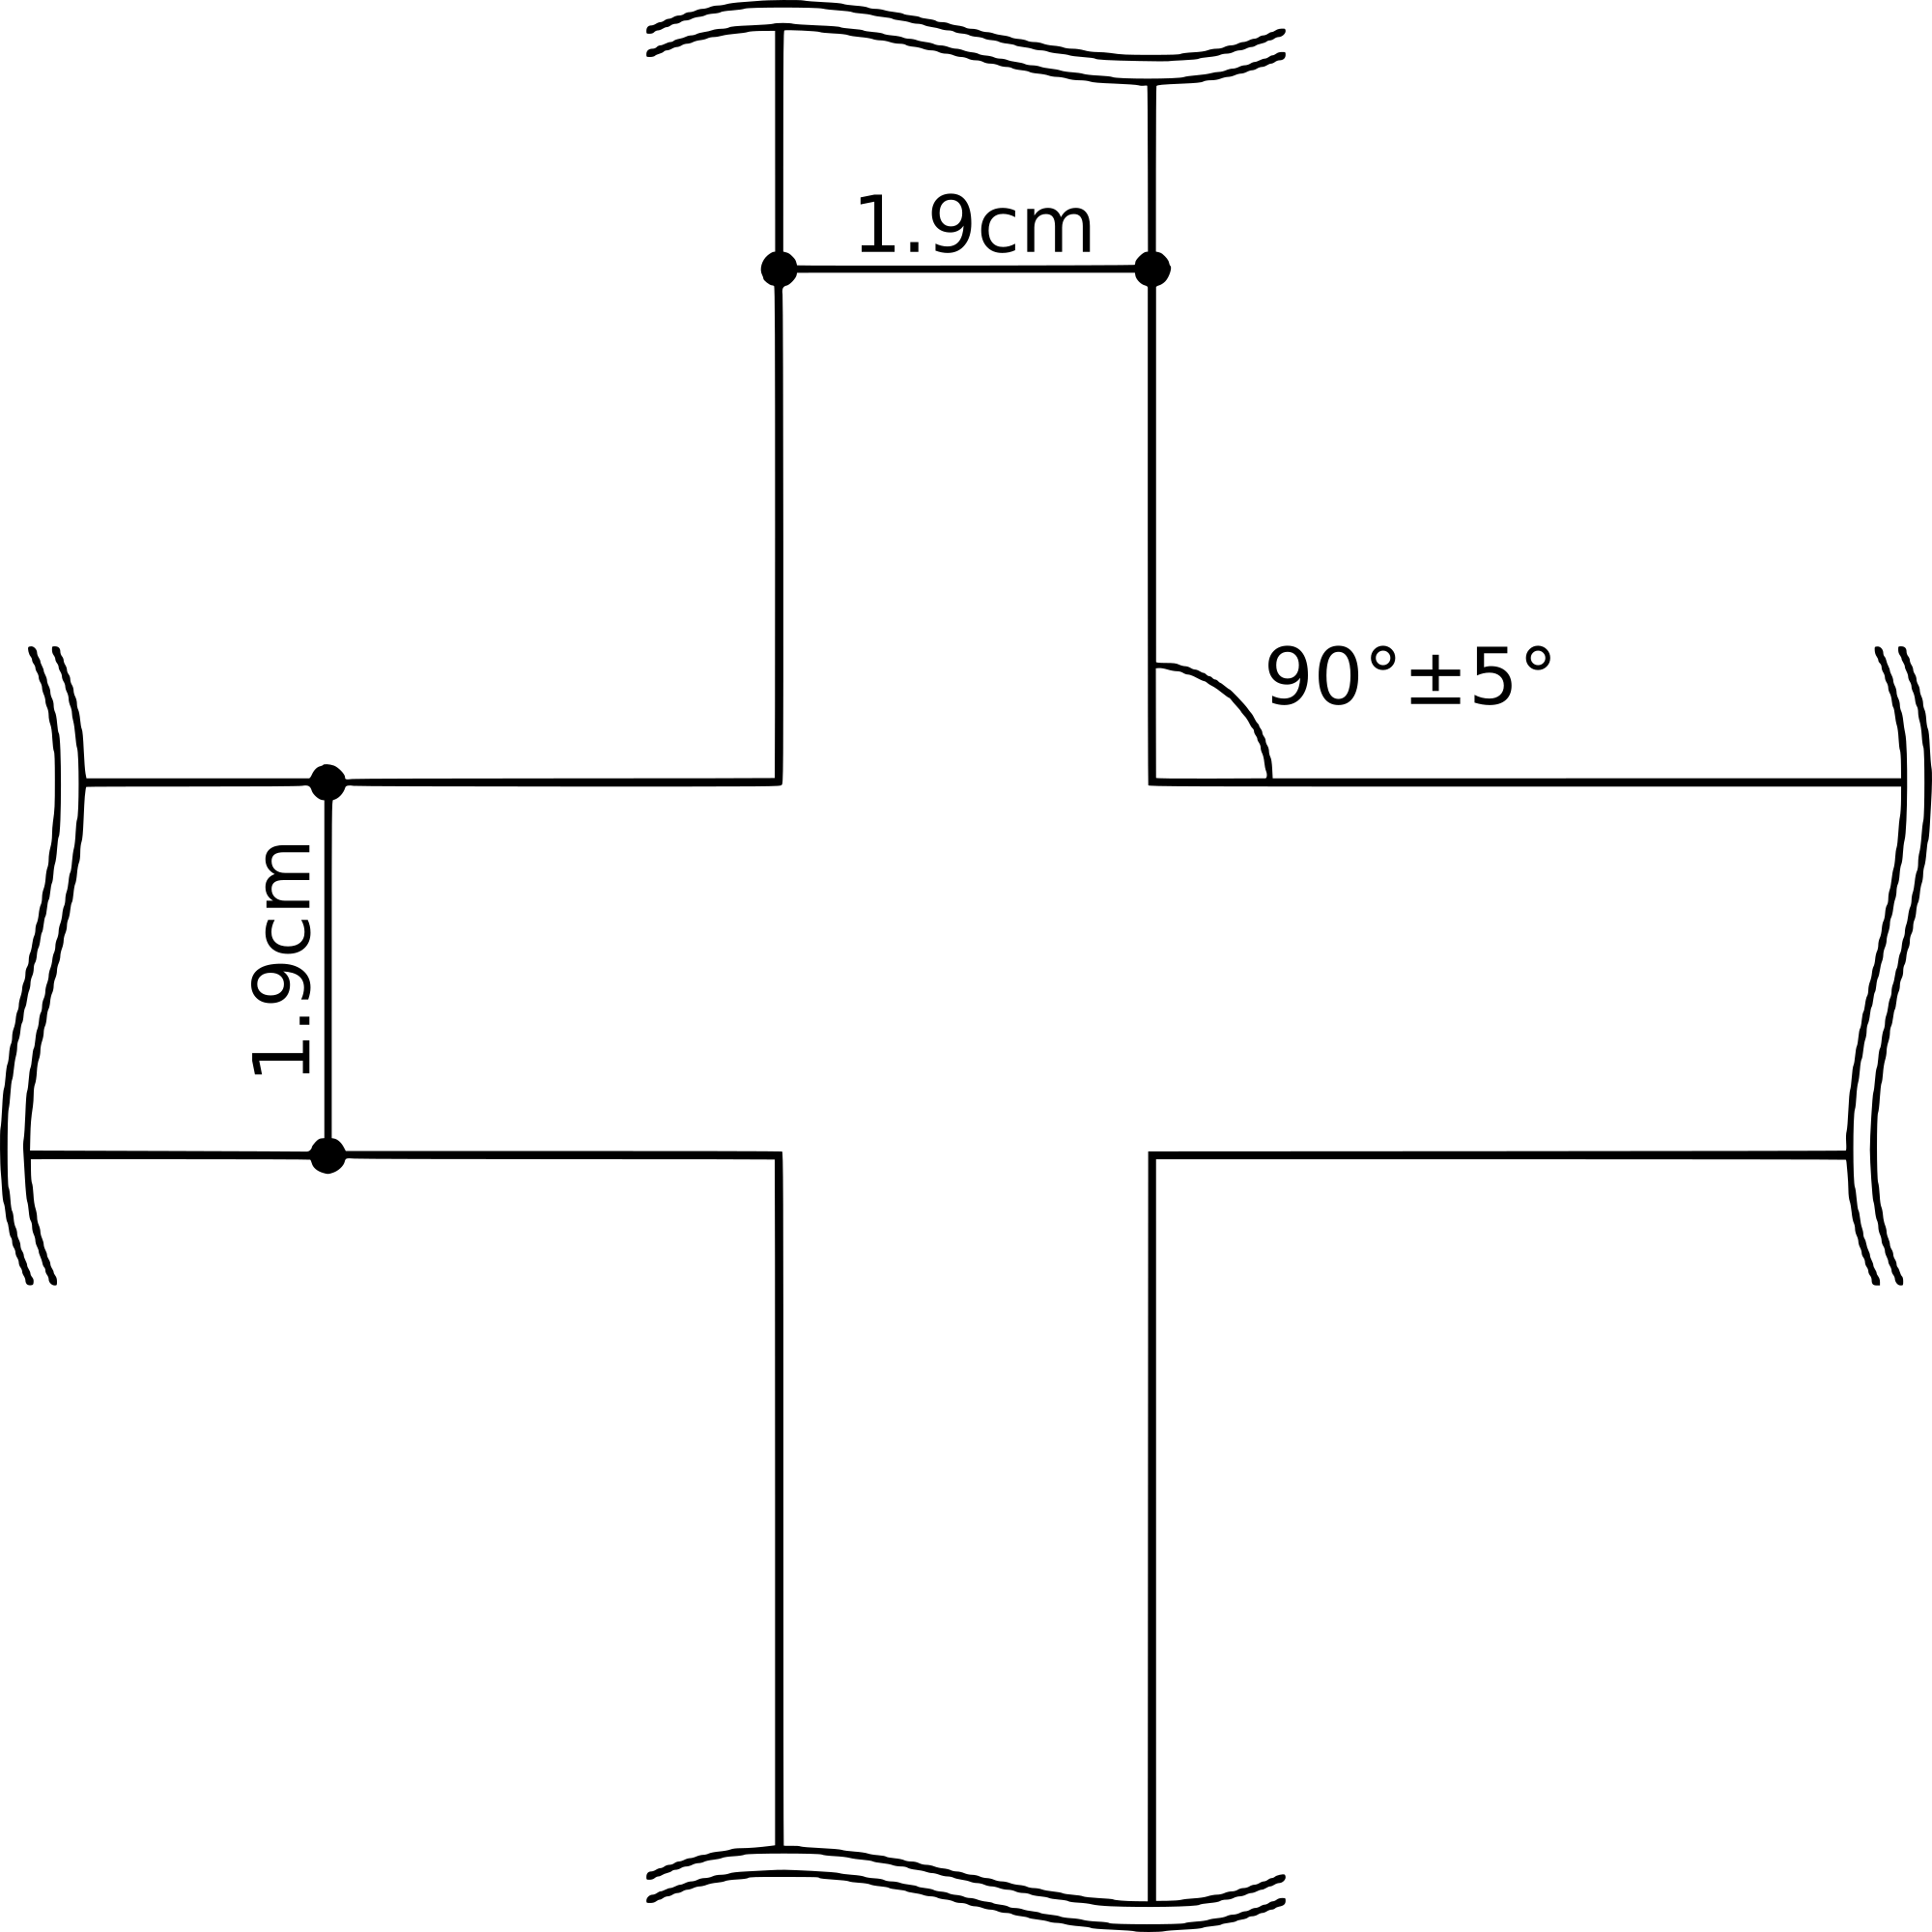
\includegraphics[width=0.6\linewidth]{./images/rules/figure3.png}
  \caption{Intersección}
  \figlabel{intersection}
\end{figure}

\begin{figure}[H]
  \centering
  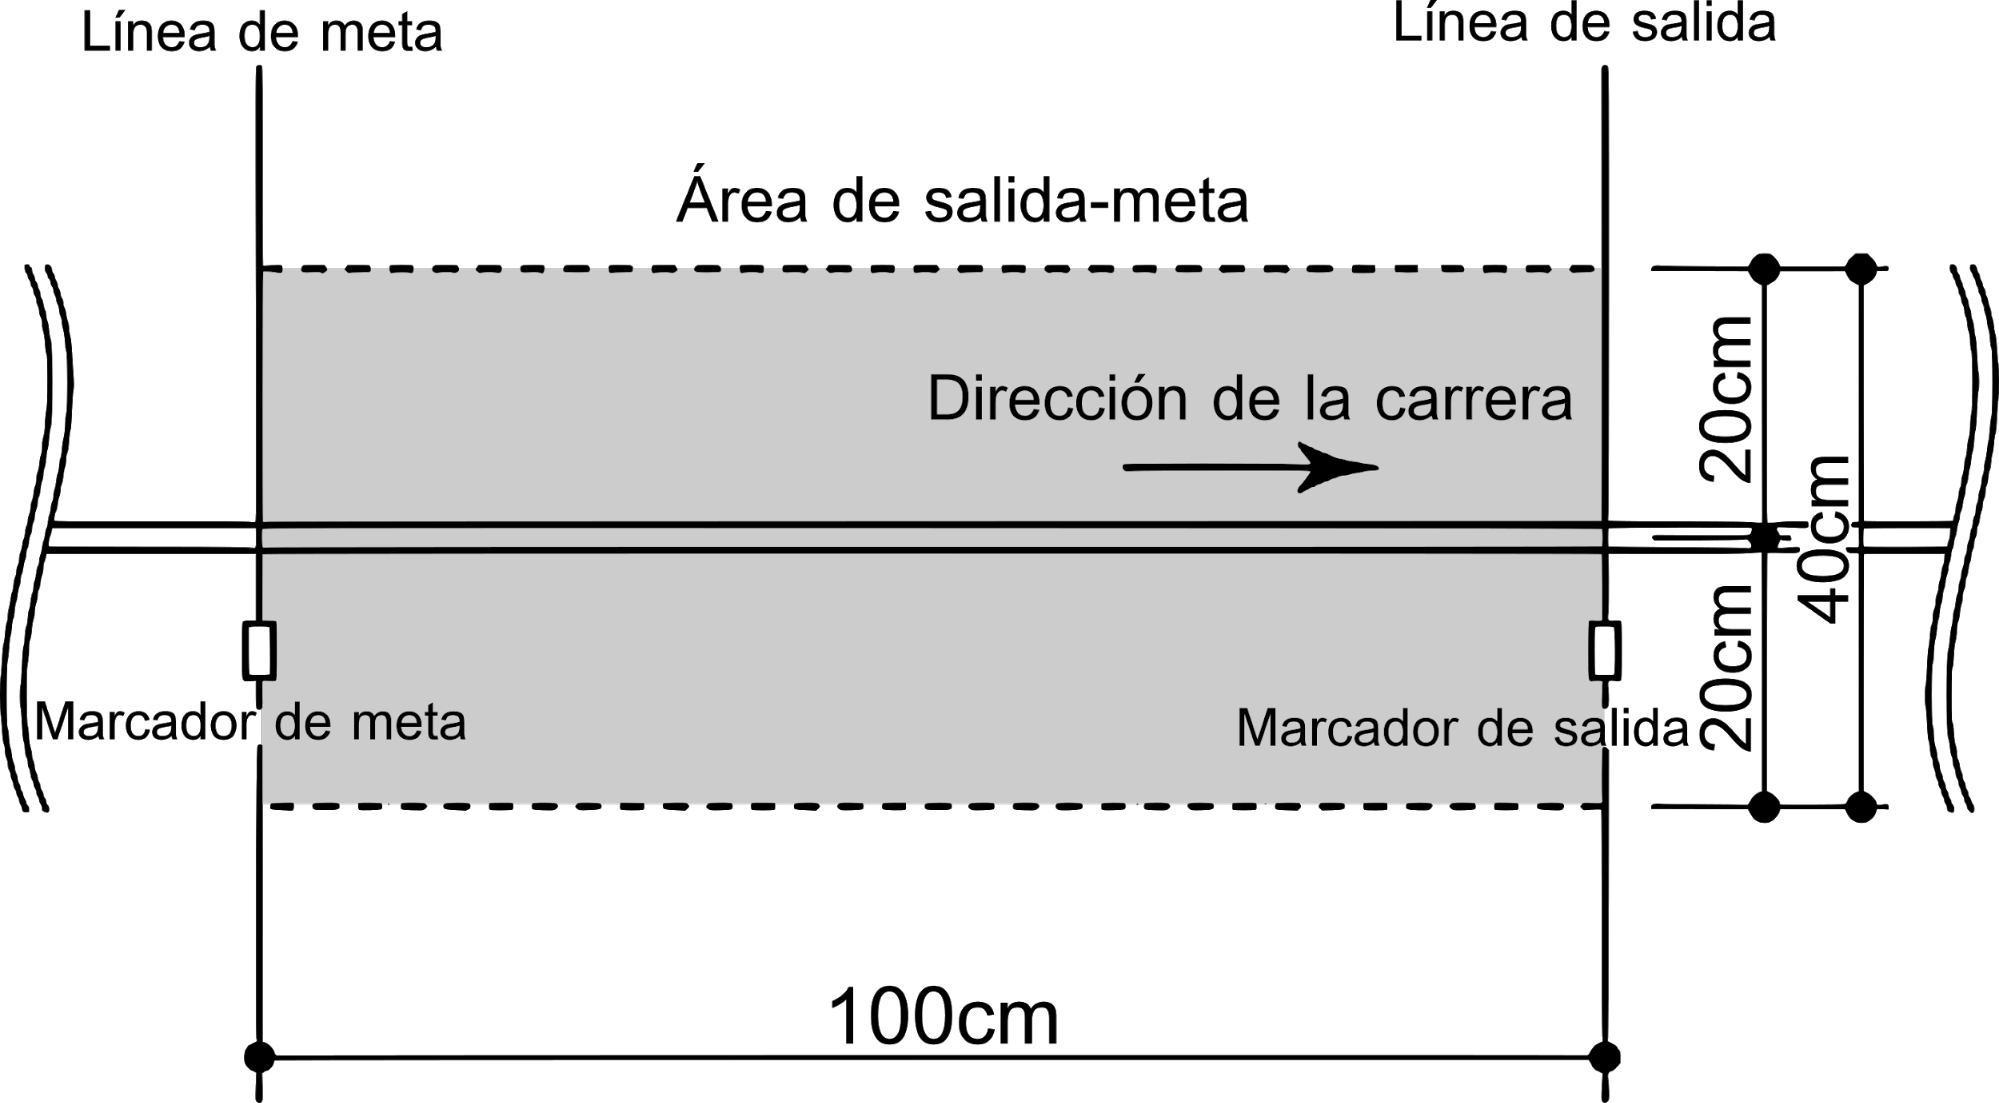
\includegraphics[width=0.6\linewidth]{./images/rules/figure4.png}
  \caption{Área de Salida-Meta}
  \figlabel{gate_area1}
\end{figure}

\begin{figure}[H]
  \centering
  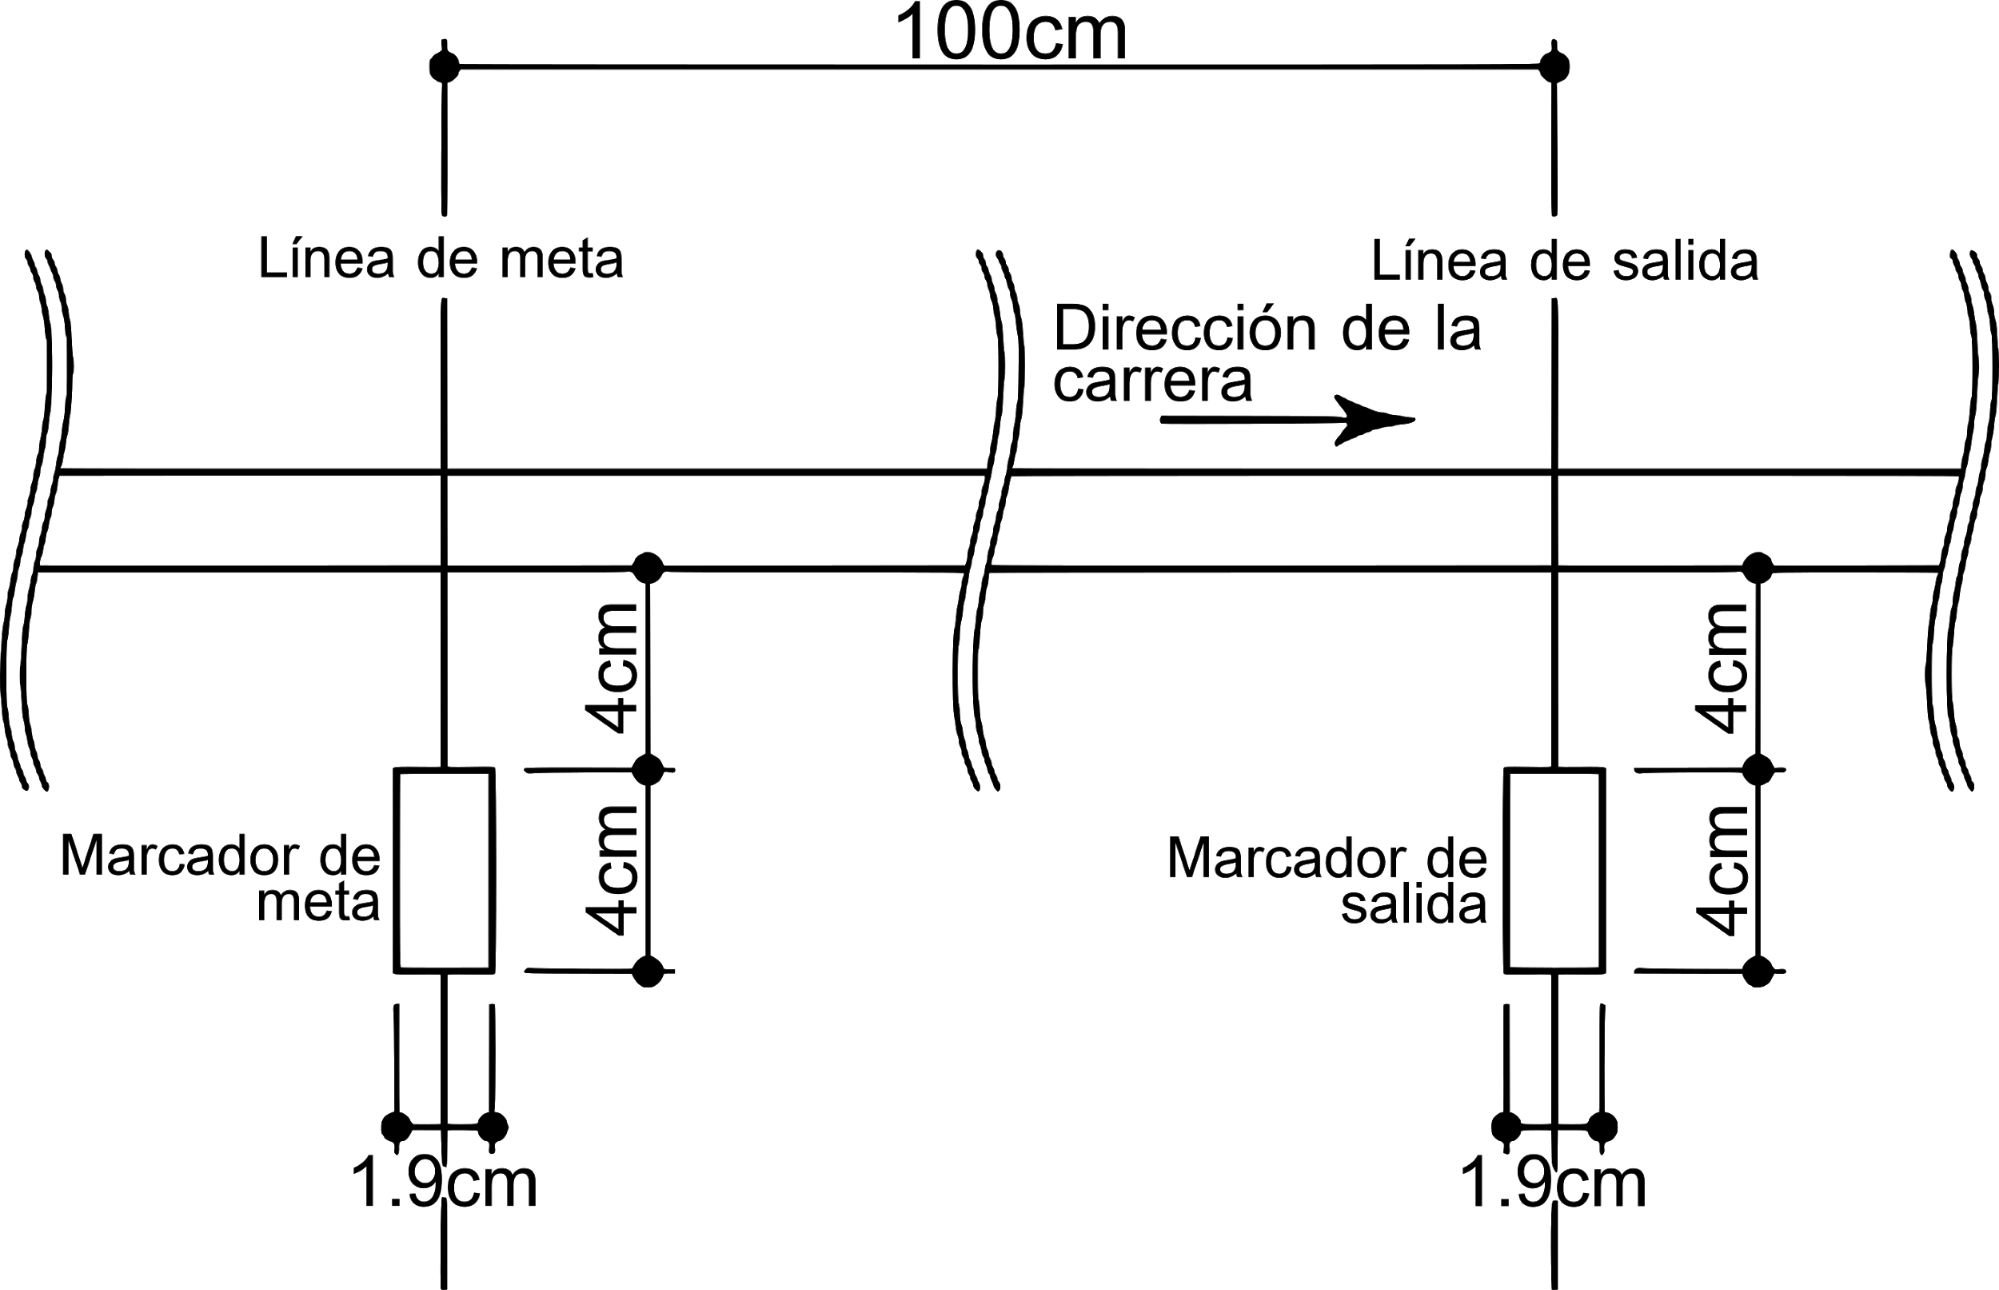
\includegraphics[width=0.6\linewidth]{./images/rules/figure5.png}
  \caption{Marcadores de Salida-Meta}
  \figlabel{gate_area2}
\end{figure}

\begin{figure}[H]
  \centering
  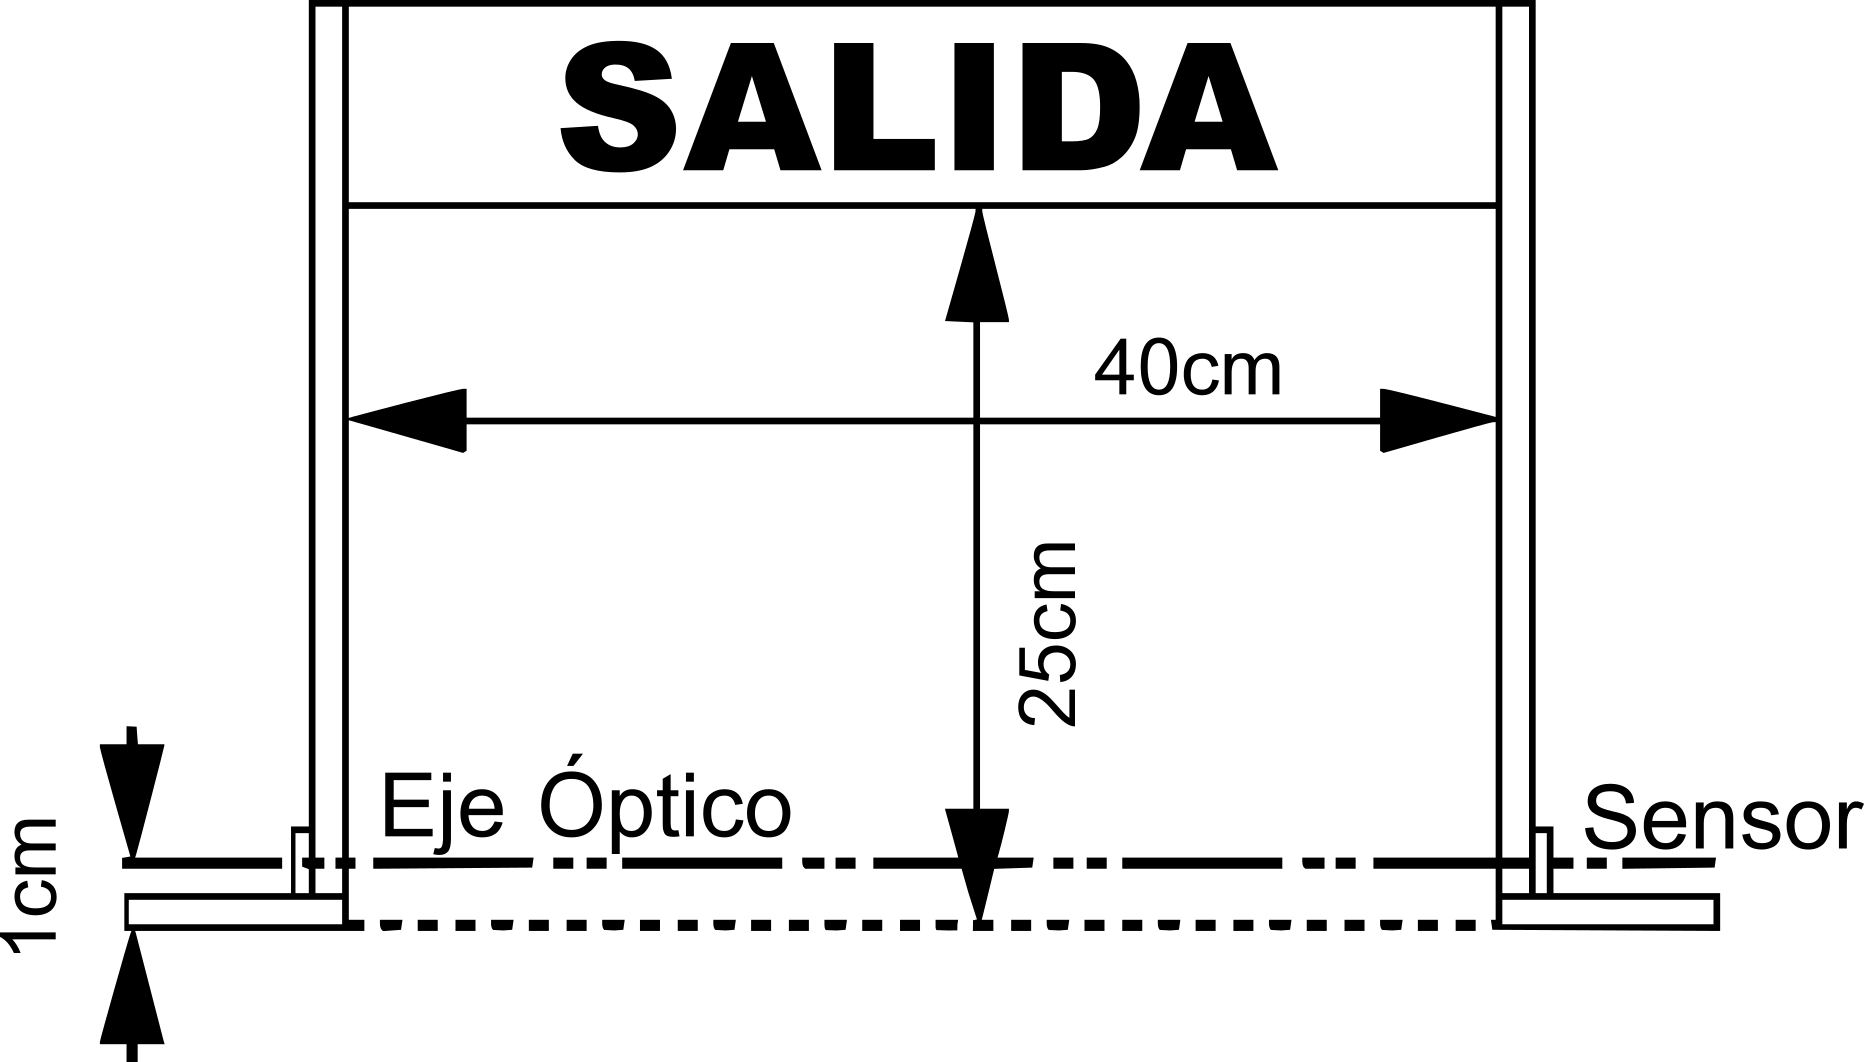
\includegraphics[width=0.6\linewidth]{./images/rules/figure6.png}
  \caption{Portal de Salida-Meta}
  \figlabel{gate}
\end{figure}



\end{document}
